% -*- coding: utf-8 -*-
%-------------------------designed by zcf--------------
\documentclass[UTF8,a4paper,10pt]{ctexart}
\usepackage[left=3.17cm, right=3.17cm, top=2.74cm, bottom=2.74cm]{geometry}
\usepackage{amsmath}
\usepackage{graphicx,subfig}
\usepackage{float}
\usepackage{cite}
\usepackage{caption}
\usepackage{enumerate}
\usepackage{booktabs} %表格
\usepackage{multirow}
\newcommand{\tabincell}[2]{\begin{tabular}{@{}#1@{}}#2\end{tabular}}  %表格强制换行
%-------------------------字体设置--------------
% \usepackage{times} 
\usepackage{ctex}
\setCJKmainfont[ItalicFont=Noto Sans CJK SC Bold, BoldFont=Noto Serif CJK SC Black]{Noto Serif CJK SC}
\newcommand{\yihao}{\fontsize{26pt}{36pt}\selectfont}           % 一号, 1.4 倍行距
\newcommand{\erhao}{\fontsize{22pt}{28pt}\selectfont}          % 二号, 1.25倍行距
\newcommand{\xiaoer}{\fontsize{18pt}{18pt}\selectfont}          % 小二, 单倍行距
\newcommand{\sanhao}{\fontsize{16pt}{24pt}\selectfont}  %三号字
\newcommand{\xiaosan}{\fontsize{15pt}{22pt}\selectfont}        % 小三, 1.5倍行距
\newcommand{\sihao}{\fontsize{14pt}{21pt}\selectfont}            % 四号, 1.5 倍行距
\newcommand{\banxiaosi}{\fontsize{13pt}{19.5pt}\selectfont}    % 半小四, 1.5倍行距
\newcommand{\xiaosi}{\fontsize{12pt}{18pt}\selectfont}            % 小四, 1.5倍行距
\newcommand{\dawuhao}{\fontsize{11pt}{11pt}\selectfont}       % 大五号, 单倍行距
\newcommand{\wuhao}{\fontsize{10.5pt}{15.75pt}\selectfont}    % 五号, 单倍行距
%-------------------------章节名----------------
\usepackage{ctexcap} 
\CTEXsetup[name={,、},number={ \chinese{section}}]{section}
\CTEXsetup[name={（,）},number={\chinese{subsection}}]{subsection}
\CTEXsetup[name={,.},number={\arabic{subsubsection}}]{subsubsection}
%-------------------------页眉页脚--------------
\usepackage{fancyhdr}
\pagestyle{fancy}
\lhead{\kaishu \leftmark}
% \chead{}
\rhead{\kaishu 深度学习原理实验报告}%加粗\bfseries 
\lfoot{}
\cfoot{\thepage}
\rfoot{}
\renewcommand{\headrulewidth}{0.1pt}  
\renewcommand{\footrulewidth}{0pt}%去掉横线
\newcommand{\HRule}{\rule{\linewidth}{0.5mm}}%标题横线
\newcommand{\HRulegrossa}{\rule{\linewidth}{1.2mm}}
%-----------------------伪代码------------------
\usepackage{algorithm}  
\usepackage{algorithmicx}  
\usepackage{algpseudocode}  
\floatname{algorithm}{Algorithm}  
\renewcommand{\algorithmicrequire}{\textbf{Input:}}  
\renewcommand{\algorithmicensure}{\textbf{Output:}} 
\usepackage{lipsum}  
\makeatletter
\newenvironment{breakablealgorithm}
  {% \begin{breakablealgorithm}
  \begin{center}
     \refstepcounter{algorithm}% New algorithm
     \hrule height.8pt depth0pt \kern2pt% \@fs@pre for \@fs@ruled
     \renewcommand{\caption}[2][\relax]{% Make a new \caption
      {\raggedright\textbf{\ALG@name~\thealgorithm} ##2\par}%
      \ifx\relax##1\relax % #1 is \relax
         \addcontentsline{loa}{algorithm}{\protect\numberline{\thealgorithm}##2}%
      \else % #1 is not \relax
         \addcontentsline{loa}{algorithm}{\protect\numberline{\thealgorithm}##1}%
      \fi
      \kern2pt\hrule\kern2pt
     }
  }{% \end{breakablealgorithm}
     \kern2pt\hrule\relax% \@fs@post for \@fs@ruled
  \end{center}
  }
\makeatother
%------------------------代码-------------------
\usepackage{xcolor} 
\usepackage{listings} 
\lstset{ 
breaklines,%自动换行
basicstyle=\small,
escapeinside=``,
keywordstyle=\color{ blue!70} \bfseries,
commentstyle=\color{red!50!green!50!blue!50},% 
stringstyle=\ttfamily,% 
extendedchars=false,% 
linewidth=\textwidth,% 
numbers=left,% 
numberstyle=\tiny \color{blue!50},% 
frame=trbl% 
rulesepcolor= \color{ red!20!green!20!blue!20},
columns=fullflexible,
keepspaces=true,
literate={-}{{-}}1
}
%------------超链接----------
\usepackage[colorlinks,linkcolor=black,anchorcolor=blue,citecolor=black,urlcolor=blue]{hyperref}
%------------------------TODO-------------------
\usepackage{enumitem,amssymb}
\newlist{todolist}{itemize}{2}
\setlist[todolist]{label=$\square$}
% for check symbol 
\usepackage{pifont}
\newcommand{\cmark}{\ding{51}}%
\newcommand{\xmark}{\ding{55}}%
\newcommand{\done}{\rlap{$\square$}{\raisebox{2pt}{\large\hspace{1pt}\cmark}}\hspace{-2.5pt}}
\newcommand{\wontfix}{\rlap{$\square$}{\large\hspace{1pt}\xmark}}
%------------------------水印-------------------
\usepackage{tikz}
\usepackage{xcolor}
\usepackage{eso-pic}

\newcommand{\watermark}[3]{\AddToShipoutPictureBG{
\parbox[b][\paperheight]{\paperwidth}{
\vfill%
\centering%
\tikz[remember picture, overlay]%
  \node [rotate = #1, scale = #2] at (current page.center)%
    {\textcolor{gray!80!cyan!30!magenta!30}{#3}};
\vfill}}}



%———————————————————————————————————————————正文———————————————————————————————————————————————
%----------------------------------------------
\begin{document}
\begin{titlepage}
    \begin{center}
    
\includegraphics[width=0.8\textwidth]{NKU.png}\\[1cm]    
    \textsc{\Huge \kaishu{\textbf{南\ \ \ \ \ \ 开\ \ \ \ \ \ 大\ \ \ \ \ \ 学}} }\\[0.9cm]
    \textsc{\huge \kaishu{\textbf{数\ \ 学\ \ 科\ \ 学\ \ 学 \ \ 院}}}\\[0.5cm]
    \textsc{\Large \textbf{深度学习原理实验报告}}\\[0.8cm]
    \HRule \\[0.9cm]
    { \LARGE \bfseries MNIST数据集手写数字识别}\\[0.4cm]
    \HRule \\[2.0cm]
    \centering
    \textsc{\LARGE 谢 \ 博\kaishu{\ \ \ \ }}\\[0.5cm]
    \textsc{\LARGE \kaishu{年级\ :\ 2024级}}\\[0.5cm]
    \textsc{\LARGE \kaishu{专业\ :\ 数学与人工智能}}\\[0.5cm]
    \textsc{\LARGE \kaishu{指导教师\ :\ 刘晓滨}}\\[0.5cm]
    \vfill
    {\Large \today}
    \end{center}
\end{titlepage}
%-------------摘------要--------------
\newpage
\thispagestyle{empty}
\renewcommand{\abstractname}{\kaishu \sihao \textbf{摘要}}
\begin{abstract}
本实验基于 PyTorch 构建并训练一个卷积神经网络，用于完成 MNIST 手写数字识别任务。实验围绕数据加载与预处理、网络结构设计、模型训练、测试评估和结果可视化展开。模型输入为 $1\times28\times28$ 的灰度图像，主体结构包含两层卷积层和两层全连接层，并使用 ReLU 激活函数、最大池化和 log softmax 输出完成多分类建模。训练阶段采用 Adam 优化器和负对数似然损失函数，在 20 个 epoch 后，模型测试准确率达到 99.11\%。实验结果表明，卷积神经网络能够有效提取手写数字图像中的局部空间特征，并在 MNIST 分类任务上取得较好的识别效果。
本次作业相关代码已上传至github，仓库地址为 \url{https://github.com/Zemiss/MnistCNN-Coursework}

\noindent\textbf{关键字：}MNIST；卷积神经网络；PyTorch；手写数字识别；深度学习
\end{abstract}
%----------------------------------------------------------------
\tableofcontents
%----------------------------------------------------------------
\newpage
\watermark{60}{10}{NKU}
\setcounter{page}{1}
\section{实验目的}
本实验使用 PyTorch 构建卷积神经网络，对 MNIST 手写数字图像进行分类识别。实验目标是完成从数据加载、模型定义、训练优化、测试评估到结果可视化的完整流程，并观察损失函数和准确率随训练轮数变化的趋势。

通过本实验，可以理解卷积层、池化层、全连接层和激活函数在图像分类中的作用，掌握使用 \texttt{DataLoader} 组织图像数据、使用 Adam 优化器训练神经网络、使用测试集准确率评估模型泛化能力的方法。同时，本实验也训练了将实验代码、指标文件和可视化结果整理为规范实验报告的能力。

\section{实验原理}
\subsection{MNIST 数据集}
MNIST 是经典的手写数字识别数据集，包含数字 0 到 9 共 10 个类别。每张样本图像为单通道灰度图，尺寸为 $28\times28$。本项目使用 \texttt{torchvision.datasets.MNIST} 自动加载数据，其中训练集包含 60000 张图像，测试集包含 10000 张图像。

在输入模型前，图像首先通过 \texttt{transforms.ToTensor()} 转换为张量，并将像素值缩放到 0 到 1。随后使用 \texttt{transforms.Normalize((0.1307,), (0.3081,))} 按 MNIST 数据集的均值和标准差进行标准化。标准化可以使输入分布更加稳定，有助于模型训练。

\subsection{卷积神经网络原理}
卷积神经网络适合处理图像数据。卷积层通过局部连接和权值共享提取图像中的笔画、边缘和局部结构特征。池化层通过下采样降低特征图尺寸，并增强模型对局部位置变化的鲁棒性。全连接层则将卷积层提取到的特征映射到具体类别。

本实验采用的模型为 \texttt{ConvNet}。模型输入为 $1\times28\times28$ 的灰度图像，输出为 10 个类别的对数概率。网络包含两层卷积层和两层全连接层，结构如表 \ref{tab:model} 所示。

\begin{table}[!htbp]
  \centering
  \begin{tabular}{ccc}
  \toprule
  层次 & 操作 & 输出形状\\
  \midrule
  输入 & MNIST 灰度图像 & $1\times28\times28$\\
  Conv1 & $5\times5$ 卷积，10 个通道，ReLU，$2\times2$ 最大池化 & $10\times12\times12$\\
  Conv2 & $3\times3$ 卷积，20 个通道，ReLU & $20\times10\times10$\\
  Flatten & 展平特征图 & 2000\\
  FC1 & 全连接层，ReLU & 500\\
  FC2 & 全连接层 & 10\\
  输出 & log softmax & 10\\
  \bottomrule
  \end{tabular}
  \caption{卷积神经网络结构}
  \label{tab:model}
\end{table}

\subsection{损失函数与评价指标}
模型最后一层使用 \texttt{log\_softmax} 输出各类别的对数概率，因此训练时采用负对数似然损失函数 \texttt{F.nll\_loss}。对于单个样本，若真实类别为 $y$，模型对该类别输出的对数概率为 $\log p_y$，则损失为：
\begin{align}
  L = -\log p_y
\end{align}

模型分类性能使用准确率衡量。准确率定义为预测正确样本数与总样本数的比值：
\begin{align}
  Accuracy = \frac{N_{correct}}{N_{total}}
\end{align}

\section{实验步骤}
\subsection{环境配置}
本项目使用 Python 3.11 和 PyTorch 实现。主要依赖包括 \texttt{torch}、\texttt{torchvision}、\texttt{pandas}、\texttt{matplotlib}、\texttt{Pillow} 和 \texttt{PyYAML}。环境配置命令如下：
\begin{lstlisting}[title=环境配置命令,frame=trbl,language={}]
conda create -n mnist-cnn python=3.11 -y
pip install -r requirements.txt
\end{lstlisting}

\subsection{项目组织}
项目中，训练脚本负责模型训练、指标记录和图像保存，测试脚本负责加载模型并执行预测。模型文件定义卷积神经网络，工具文件封装训练、测试和绘图函数，配置文件保存默认参数。主要目录结构如下：
\begin{lstlisting}[title=项目目录结构,frame=trbl,language={}]
.
|-- configs/
|   |-- default.yaml
|-- src/
|   |-- config.py
|   |-- model.py
|   |-- utils.py
|-- train.py
|-- test.py
|-- requirements.txt
|-- model/
|   |-- mnist_cnn.pth
|-- outputs/
    |-- metrics.csv
    |-- loss_curve.png
    |-- accuracy_curve.png
    |-- sample_ground_truth.png
    |-- sample_predictions.png
\end{lstlisting}

\subsection{训练流程}
实验默认批大小为 512，训练轮数为 20，随机种子为 1，优化器为 Adam，学习率为 0.001。训练脚本会优先使用 CUDA 设备；如果没有可用 GPU，则自动使用 CPU。每个 batch 中，脚本依次执行前向传播、损失计算、反向传播和参数更新。每个 epoch 结束后，脚本在测试集上计算平均损失和准确率。

模型保存策略为最佳测试准确率保存。只有当当前 epoch 的测试准确率高于历史最佳值时，脚本才会将权重保存到 \texttt{model/mnist\_cnn.pth}。训练结束后，脚本会保存 \texttt{metrics.csv}、损失曲线、准确率曲线、真实标签样例和预测样例。

训练命令如下：
\begin{lstlisting}[title=训练命令,frame=trbl,language={}]
python train.py
\end{lstlisting}

\subsection{测试流程}
训练完成后，可以使用 \texttt{test.py} 加载保存的模型权重进行测试。若直接使用 MNIST 测试集，可执行如下命令：
\begin{lstlisting}[title=使用 MNIST 测试集测试,frame=trbl,language={}]
python test.py --test-data-dir data --model-path model\mnist_cnn.pth --use-mnist --num-samples 20
\end{lstlisting}

测试脚本也支持读取自定义图片文件夹，并逐张输出预测类别和对应概率。支持的图片格式包括 \texttt{.png}、\texttt{.jpg}、\texttt{.jpeg} 和 \texttt{.bmp}。使用自定义图片文件夹时，可执行如下命令：
\begin{lstlisting}[title=使用图片文件夹测试,frame=trbl,language={}]
python test.py --test-data-dir path\to\digit_images --model-path model\mnist_cnn.pth --no-use-mnist
\end{lstlisting}

\section{程序代码}
\subsection{模型定义代码}
核心网络定义位于 \texttt{src/model.py}。模型先通过两层卷积提取图像特征，再将特征展平并输入两层全连接层，最后输出 10 个类别的对数概率。
\begin{lstlisting}[title=ConvNet 模型定义,frame=trbl,language={Python}]
class ConvNet(nn.Module):
    def __init__(self):
        super().__init__()
        self.conv1 = nn.Conv2d(1, 10, 5)
        self.conv2 = nn.Conv2d(10, 20, 3)
        self.fc1 = nn.Linear(20 * 10 * 10, 500)
        self.fc2 = nn.Linear(500, 10)

    def forward(self, x):
        in_size = x.size(0)
        out = self.conv1(x)
        out = F.relu(out)
        out = F.max_pool2d(out, 2, 2)
        out = self.conv2(out)
        out = F.relu(out)
        out = out.view(in_size, -1)
        out = self.fc1(out)
        out = F.relu(out)
        out = self.fc2(out)
        return F.log_softmax(out, dim=1)
\end{lstlisting}

\subsection{训练代码}
训练过程封装在 \texttt{src/utils.py} 的 \texttt{train\_epoch} 函数中。每个 batch 先清空梯度，再计算模型输出和损失，随后执行反向传播和优化器更新。
\begin{lstlisting}[title=单轮训练核心代码,frame=trbl,language={Python}]
for batch_idx, (data, target) in enumerate(train_loader):
    data = data.to(device)
    target = target.to(device)

    optimizer.zero_grad()
    output = model(data)
    loss = F.nll_loss(output, target)
    loss.backward()
    optimizer.step()

    pred = output.data.max(1, keepdim=True)[1]
    correct += pred.eq(target.data.view_as(pred)).sum().item()
\end{lstlisting}

\subsection{测试评价代码}
测试过程在不计算梯度的条件下执行。脚本将模型切换到评价模式，累计测试集损失和预测正确样本数，并计算测试准确率。
\begin{lstlisting}[title=测试评价核心代码,frame=trbl,language={Python}]
model.eval()
test_loss = 0.0
correct = 0

for data, target in test_loader:
    data = data.to(device)
    target = target.to(device)
    output = model(data)
    test_loss += F.nll_loss(output, target, reduction="sum").item()
    pred = output.data.max(1, keepdim=True)[1]
    correct += pred.eq(target.data.view_as(pred)).sum().item()

test_loss /= len(test_loader.dataset)
test_acc = correct / len(test_loader.dataset)
\end{lstlisting}

\section{实验结果显示}
\subsection{真实标签样例}
图 \ref{fig:ground_truth} 展示了测试集中部分手写数字样例及其真实标签。可以看到，MNIST 图像均为灰度图，数字形态存在一定差异，这要求模型能够学习具有鲁棒性的局部笔画特征。
\begin{figure}[H]
    \centering
    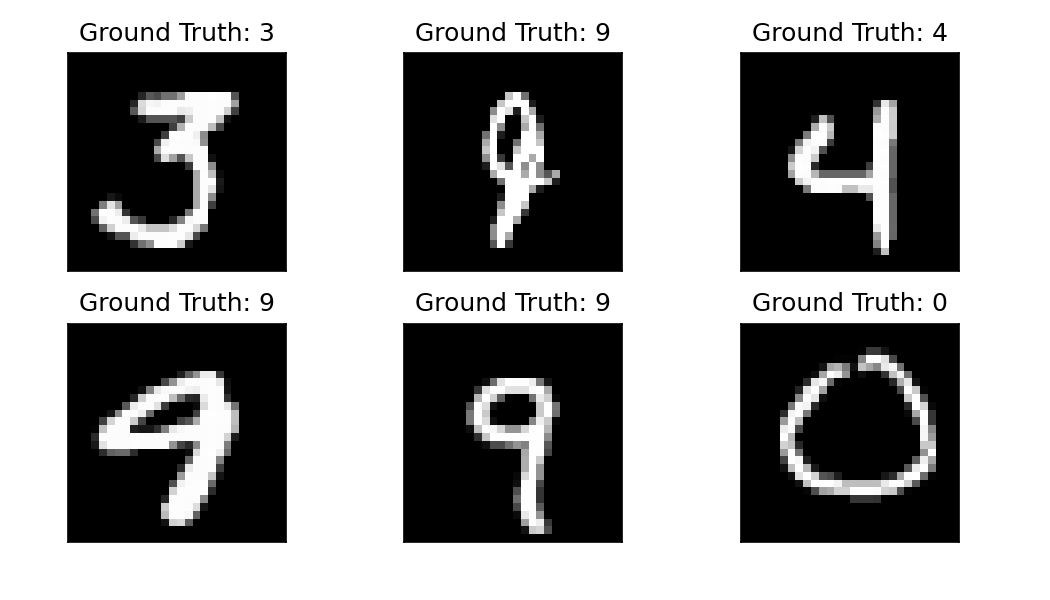
\includegraphics[width=0.75\textwidth]{../../outputs/sample_ground_truth.png}
    \caption{MNIST 测试样例真实标签}
    \label{fig:ground_truth}
\end{figure}

\subsection{训练指标}
本次训练共运行 20 个 epoch。训练损失从第 1 轮的 0.3273 降至第 20 轮的 0.0011，训练准确率从 90.91\% 提升到 99.98\%。测试损失从第 1 轮的 0.1155 降至第 20 轮的 0.0379，测试准确率从 96.33\% 提升到 99.11\%。最高测试准确率出现在第 20 轮，为 99.11\%。

\begin{table}[!htbp]
  \centering
  \begin{tabular}{ccccc}
  \toprule
  Epoch & Train Loss & Train Acc & Test Loss & Test Acc\\
  \midrule
  1 & 0.3273 & 90.91\% & 0.1155 & 96.33\%\\
  5 & 0.0340 & 98.92\% & 0.0395 & 98.73\%\\
  10 & 0.0084 & 99.76\% & 0.0374 & 98.92\%\\
  15 & 0.0037 & 99.90\% & 0.0375 & 99.10\%\\
  20 & 0.0011 & 99.98\% & 0.0379 & 99.11\%\\
  \bottomrule
  \end{tabular}
  \caption{部分 epoch 的训练与测试指标}
  \label{tab:metrics}
\end{table}

\subsection{损失曲线}
\begin{figure}[H]
    \centering
    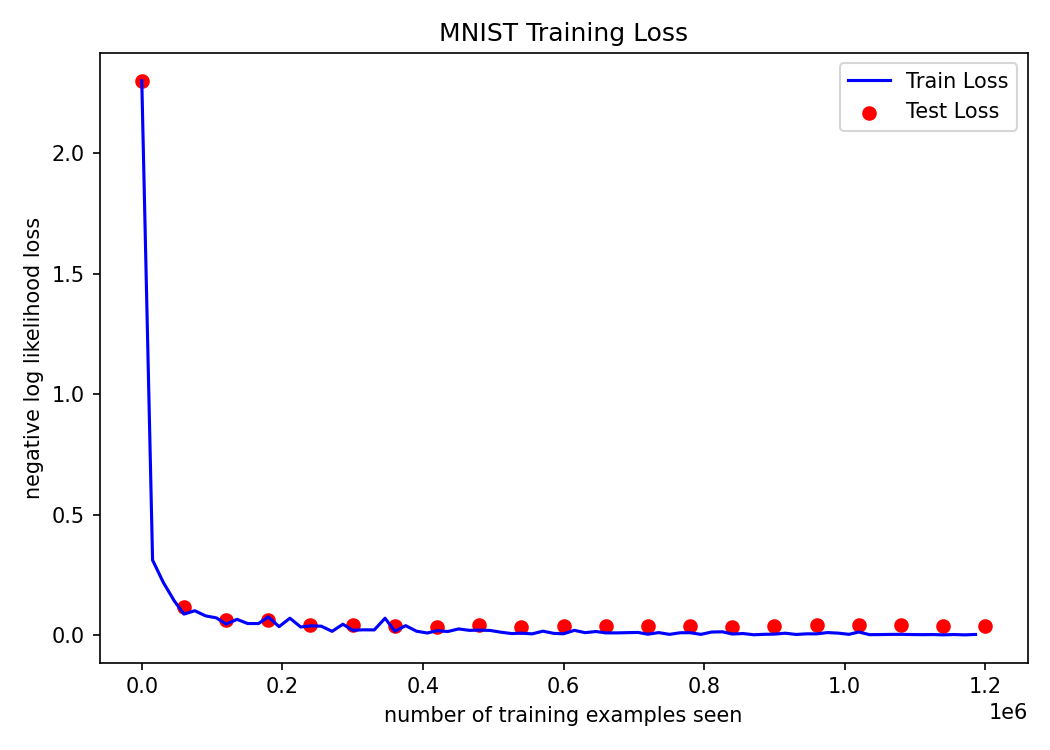
\includegraphics[width=0.75\textwidth]{../../outputs/loss_curve.png}
    \caption{训练损失与测试损失变化曲线}
    \label{fig:loss}
\end{figure}

\subsection{准确率曲线}
\begin{figure}[H]
    \centering
    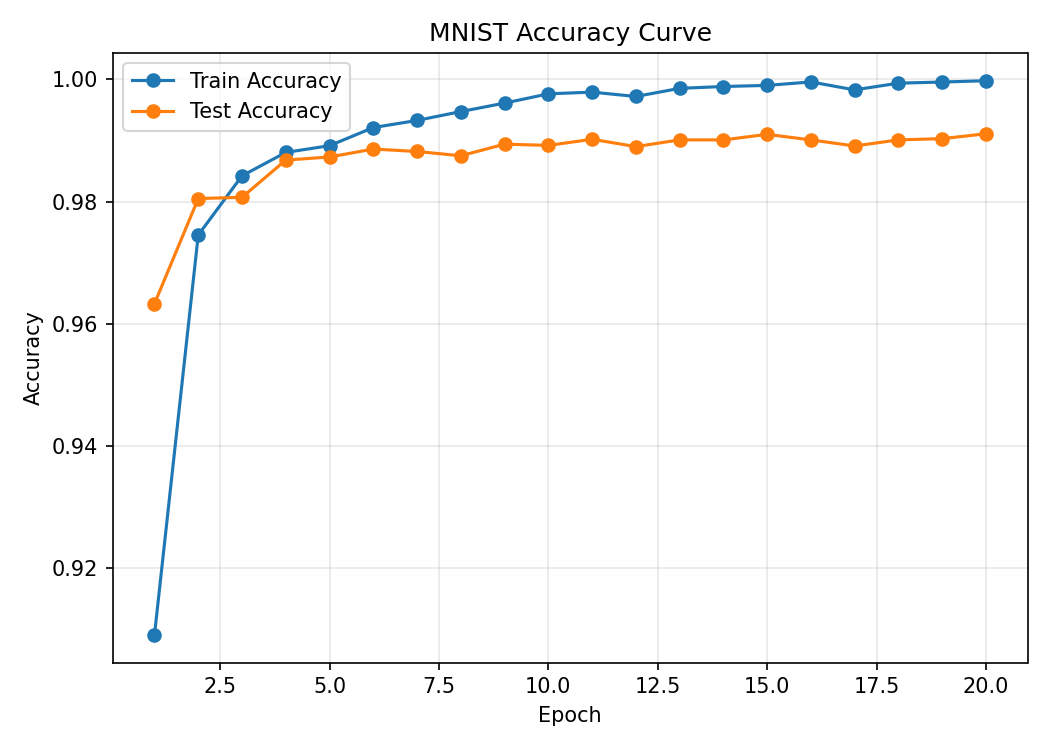
\includegraphics[width=0.75\textwidth]{../../outputs/accuracy_curve.png}
    \caption{训练准确率与测试准确率变化曲线}
    \label{fig:accuracy}
\end{figure}

\subsection{预测样例}
\begin{figure}[H]
    \centering
    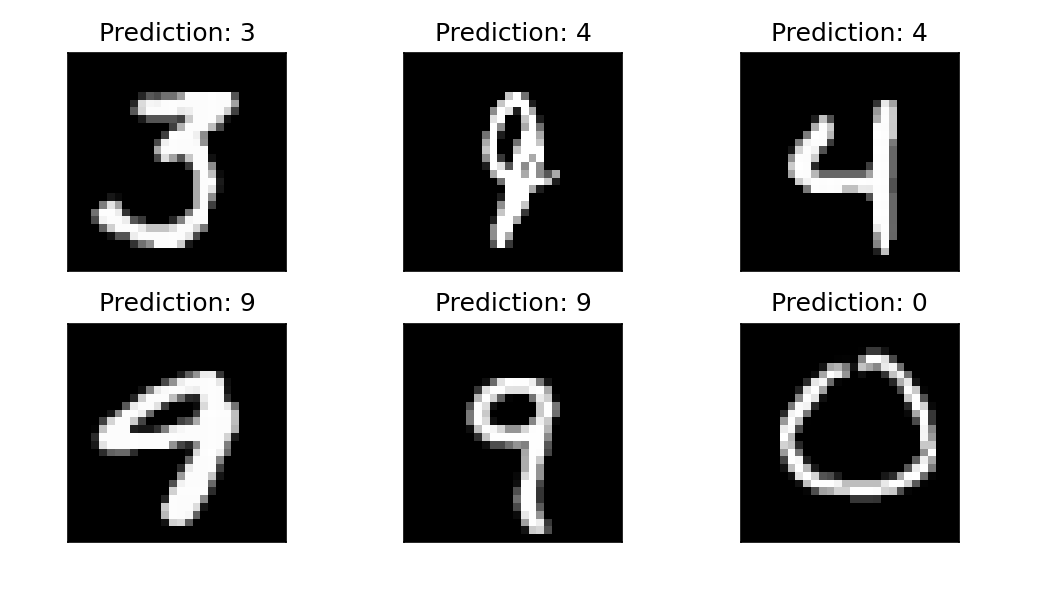
\includegraphics[width=0.75\textwidth]{../../outputs/sample_predictions.png}
    \caption{MNIST 测试样例预测结果}
    \label{fig:predictions}
\end{figure}

\section{实验分析总结}
从表 \ref{tab:metrics} 和图 \ref{fig:loss} 可以看出，模型在前几个 epoch 内快速收敛。第 5 轮时训练准确率已经达到 98.92\%，测试准确率达到 98.73\%。这说明卷积网络能够较快学习 MNIST 图像中的主要判别特征。随着训练继续进行，训练损失持续下降，训练准确率逐步接近 100\%。

图 \ref{fig:accuracy} 显示，测试准确率在第 6 轮后基本稳定在 98.8\% 以上，并在后续训练中缓慢提升到 99.11\%。训练准确率和测试准确率之间存在一定差距，这是模型在训练样本和未见样本上表现不同造成的正常泛化误差。测试损失在训练后期存在轻微波动，说明模型已经接近收敛，继续训练对测试准确率的提升有限。

图 \ref{fig:predictions} 展示了模型在测试样例上的预测结果。训练后的卷积神经网络能够识别不同形态的手写数字，并给出与图像内容一致的类别预测。整体来看，两层卷积层和两层全连接层构成的 CNN 已经能够较好地完成 MNIST 手写数字分类任务。

本实验的不足在于模型结构较简单，未加入 dropout、数据增强或学习率调度等改进手段。若进一步扩展实验，可以比较不同优化器、学习率、batch size 和网络深度对测试准确率的影响，也可以在自定义手写数字图片上测试模型的实际泛化能力。

\newpage
\nocite{*}
\bibliographystyle{plain}
\bibliography{references}

\end{document}
